% =====================================================================
%  QSentry: A Telemetry-Driven Intelligent Security Layer for
%           Resilient Quantum Communication Networks
%
%  Springer LNCS format. Prepared for QUANCOM 2026.
%
%  BUILD:  this file needs the official Springer LNCS class files
%          (llncs.cls, splncs04.bst). They are NOT bundled here; see
%          paper/README_PAPER.md for the one-step download. Then:
%             pdflatex main && bibtex main && pdflatex main && pdflatex main
%
%  RESULTS WIRING:
%    * Tables for the PRESERVED experiments (closed-set, cross-domain,
%      open-set, dataset dimensions) are written inline below.
%    * Tables for the NEW experiments are \input from paper/tables/ and
%      figures are \includegraphics from paper/figures/. Run the pipeline
%      (scripts/run_all.sh configs/experiment/full.yaml) to regenerate
%      them with publication-scale numbers; the committed versions are
%      smoke-test placeholders so the document compiles out of the box.
% =====================================================================
\documentclass[runningheads]{llncs}

\usepackage[T1]{fontenc}
\usepackage{graphicx}
\usepackage{amsmath,amssymb}
\usepackage{booktabs}
\usepackage{multirow}
\usepackage{algorithm}
\usepackage{algorithmic}
\usepackage{xcolor}
\usepackage{hyperref}
\usepackage{url}
\graphicspath{{figures/}}
\hypersetup{hidelinks}

\begin{document}

\title{QSentry: A Telemetry-Driven Intelligent Security Layer for Resilient Quantum Communication Networks}
\titlerunning{QSentry: A Telemetry-Driven Security Layer for Quantum Networks}

\author{First Author\inst{1}\orcidID{0000-0000-0000-0000} \and
Second Author\inst{2}\orcidID{0000-0000-0000-0000}}
\authorrunning{F. Author et al.}

\institute{Affiliation One, City, Country\\
\email{first.author@example.org}
\and
Affiliation Two, City, Country\\
\email{second.author@example.org}}

\maketitle

\begin{abstract}
Twin-Field Quantum Key Distribution (TF-QKD) relaxes the repeaterless rate--distance limit and is therefore a leading candidate for the trunk links of future quantum communication networks. Its practicality, however, depends on phase stabilization, reference-light handling, and detector engineering, all of which expose an implementation attack surface that protocol-level security proofs do not cover. We argue that resilient quantum networks need an \emph{intelligent security layer} that continuously audits the optical control plane, and we present \textsc{QSentry}, a telemetry-driven design built around a deliberate separation of two tasks: closed-set recognition of known implementation attacks and open-set detection of novel ones. \textsc{QSentry} couples a strong sequence classifier with a one-class anomaly scorer and surrounds them with a trust layer that monitors calibration and converts model scores into operator-facing alarms. On a physically-grounded TF-QKD telemetry benchmark with clean, drifted, asymmetric-loss, and unknown domains ($T{\times}F = 32{\times}12$ windows), a Transformer is the strongest closed-set detector across every domain (macro-F1 $0.9990 \to 0.9384 \to 0.8686 \to 0.8993$ from clean to unknown), a hybrid quantum LSTM is competitive but not superior, and the autoencoder is most useful as a ranking-based novelty detector (ROC-AUC up to $0.85$ with high average precision) rather than as a thresholded classifier. Beyond detection accuracy we report the operational evidence an infrastructure deployment needs: calibration degrades measurably under domain shift, robustness curves quantify graceful degradation as shift severity grows, inference latency and parameter budgets are compatible with control-plane rates for the classical models but not for the simulated quantum model, and permutation analysis shows that physically-meaningful channels---phase-lock error, QBER phase, reference power, coincidence rate---carry the decisive signal. The result is a coherent, reproducible blueprint for an AI/QML security layer for resilient quantum communication networks, together with an honest account of where quantum models do and do not help in the NISQ era.
\keywords{Quantum communication networks \and Twin-Field QKD \and Intelligent security layer \and Anomaly detection \and Domain shift \and Calibration \and Quantum machine learning \and Reproducibility.}
\end{abstract}

% =====================================================================
\section{Introduction}
% =====================================================================
The long-term security of classical public-key cryptography is threatened by scalable quantum computers, which is the central motivation for the parallel transition toward post-quantum cryptography and toward quantum-secure communication at the physical layer~\cite{preskill2018quantum,shor1999polynomial,csrcNIST}. Quantum key distribution (QKD) addresses key exchange through physics rather than computational hardness, beginning with BB84 and extending through decoy-state and measurement-device-independent protocols~\cite{bb84,pns,hwang,lo2005,mdi}. Twin-Field QKD (TF-QKD) is particularly important for networking because it overcomes the repeaterless rate--distance limit that constrains earlier architectures, which makes it a natural candidate for the long trunk links of an emerging quantum internet~\cite{tfqkd,wehner2018internet,chen2021integrated}. That same practicality, however, widens the implementation surface, especially around phase stabilization, local-reference handling, and detector-side engineering.

The implementation literature is unambiguous that practical QKD is not secured by the abstract protocol alone. Detector blinding, Trojan-horse probing, wavelength-dependent beam-splitter effects, and reference-light manipulation all operate through imperfect hardware rather than through the idealized protocol model~\cite{lydersen,makarov,gisin,jain,li2011}. The recent TF-QKD wavelength-switching attack on optical phase-locked-loop (OPLL) hardware is a sharp reminder that practical security must be evaluated against the \emph{telemetry} generated by the optical control system, not only against the key-generation equations~\cite{peng}. As QKD moves from point-to-point demonstrations toward multi-node networks, this monitoring problem becomes a networking and operations problem: every node and relay produces a stream of control telemetry that must be audited in real time, and an attack on one link should be detectable, attributable, and actionable from that telemetry.

This paper takes the position that resilient quantum communication networks require an \emph{intelligent security layer}: a telemetry-driven service that sits in the control plane, distinguishes attack signatures from benign non-stationary variation, flags behaviour it has never seen, and reports calibrated, operator-usable alarms. We instantiate this position as \textsc{QSentry}. Rather than asking ``which model wins,'' we ask how to \emph{build, evaluate, and operate} such a layer, and we are deliberately careful to separate two tasks that the literature too often conflates: closed-set classification of known attacks and open-set detection of unknown ones. Conflating them produces misleading metrics and, worse, misleading operational confidence.

\paragraph{Contributions.} This work makes the following contributions.
\begin{enumerate}
\item \textbf{An intelligent security-layer design (\textsc{QSentry}).} We formulate a two-stage control-plane monitor---a closed-set sequence detector plus an open-set one-class novelty detector---wrapped in a trust layer that tracks calibration and turns scores into alarms (Section~\ref{sec:framework}). The design is explicitly positioned for resilient, multi-node quantum networks.
\item \textbf{A physically-grounded, domain-shift-aware telemetry benchmark.} We describe a TF-QKD control-telemetry generator whose phase-basis QBER channel is computed from interference physics, with clean, drift, asymmetric-loss, and unknown domains and a held-out novelty class for zero-shot evaluation (Section~\ref{sec:benchmark}). The generator, datasets, and an integrity audit are released.
\item \textbf{A correct dual-track evaluation protocol and a model audit.} We report closed-set, cross-domain, and open-set results under a leakage-free protocol that scores label recognition and novelty detection separately, and we correct an over-optimistic reading of quantum advantage (Sections~\ref{sec:setup}--\ref{sec:results}).
\item \textbf{Operational evidence for deployment.} Beyond accuracy we measure calibration under shift, robustness as a function of shift severity, inference latency and parameter budget, and per-channel importance for operator dashboards (Section~\ref{sec:results}). These are exactly the quantities an infrastructure venue needs and that prior framings omit.
\item \textbf{A reproducible bundle.} We release the full pipeline---data generation, training, evaluation, robustness, figures, tables, and the manuscript sources---so every number and figure can be regenerated end to end.
\end{enumerate}

The honest headline is operational, not triumphalist: a strong classical sequence model paired with a separate novelty detector, made trustworthy through calibration monitoring and characterized for deployment, is a credible security layer for quantum networks today; a hybrid quantum model is a viable comparator but not, in this benchmark, an empirically superior one.

% =====================================================================
\section{Background and Related Work}
% =====================================================================
\subsection{From QKD Protocols to Quantum Networks}
QKD rests on the principle that measurement disturbs quantum states, allowing two parties to bound an eavesdropper's information~\cite{bb84}. Practical systems moved from idealized single-photon assumptions toward weak coherent pulses with decoy-state analysis to suppress photon-number-splitting attacks~\cite{pns,hwang,lo2005}, while the measurement-device-independent family removed detector-side vulnerabilities by relocating measurement to an untrusted relay~\cite{mdi}. TF-QKD then broke the repeaterless loss scaling that had limited all of these, making long single-span links viable~\cite{tfqkd}. As field deployments grow into metropolitan and intercity networks~\cite{chen2021integrated,wehner2018internet,pirandola2020advances}, security must be reasoned about at the level of an operational system: protocol-level proofs are necessary but not sufficient, because the control hardware that keeps a TF-QKD link locked is itself part of the attack surface.

\subsection{Physical-Layer Attacks on Practical QKD}
The deployed attack surface is dominated by hardware imperfection. Bright-illumination and detector-control attacks force avalanche photodiodes out of Geiger mode~\cite{lydersen,makarov}; Trojan-horse probing and wavelength-dependent attacks exploit reflection and spectral mismatch in modulators and beam splitters~\cite{gisin,li2011}; and a practical review stresses that these are the normal failure mode of real systems rather than corner cases~\cite{jain}. In TF-QKD the OPLL and reference-light path are especially sensitive: the wavelength-switching attack shows that a small change in reference wavelength can raise the mean photon number appreciably without obviously breaking interference~\cite{peng}. Each of these attacks leaves a characteristic imprint on control telemetry---count statistics, reference power, visibility, phase-lock error, wavelength offset---which is precisely what a telemetry-driven monitor can learn to recognize.

\subsection{Machine Learning, Quantum Machine Learning, and Trust}
The telemetry is multivariate and temporally coupled, so sequence models are a natural fit. Self-attention is a mature sequence learner with well-understood behaviour~\cite{vaswani2017attention}, and recurrent networks remain strong baselines~\cite{hochreiter1997lstm}. Quantum machine learning offers kernels, variational circuits, and hybrid recurrent models as alternative sequence learners or anomaly detectors~\cite{rebentrost2014quantum,schuld2019quantum,havlicek2019supervised,qlstm,chen,data_reuploading,corli2024review}, but the same literature cautions against overclaiming: parameterized circuits can be hard to train, can exhibit barren plateaus, and can show generalization behaviour that resists naive capacity arguments~\cite{mcclean2018barren,cerezo2021variational,larocca2024review,gilfuster2024generalization,haug2024qfim,lu2020quantum,lu}. A security layer additionally has to be \emph{trustworthy}: its confidence must track its accuracy. We therefore draw on the calibration and out-of-distribution literature---expected calibration error and reliability diagrams~\cite{guo2017calibration,naeini2015ece}, baselines for detecting out-of-distribution inputs~\cite{hendrycks2017baseline}, reconstruction-based novelty scoring~\cite{an2015variational}, and detection-error-tradeoff analysis~\cite{martin1997det}---and bring it to bear on QKD monitoring, which to our knowledge has not been done in a domain-shift-aware way.

% =====================================================================
\section{Threat Model and Physical Telemetry}\label{sec:threat}
% =====================================================================
\subsection{Control-Plane Telemetry}
We model the control telemetry of a TF-QKD station as a multivariate time series. At time step $t$ the station emits a vector $x_t\in\mathbb{R}^{F}$ of $F=12$ physical channels: phase-lock error, phase- and time-basis QBER, interference visibility, reference (local-oscillator) power, coincidence rate, mean photon number, single-detector count rate, dark-count rate, reference wavelength offset, phase-drift rate, and timing jitter. A monitoring window is a sequence of $T=32$ such vectors, i.e.\ a tensor slice $X\in\mathbb{R}^{T\times F}$. The measured interference quality couples the relative phase error $\delta\phi_t$ and the instantaneous visibility $V_t$, so the phase-basis QBER obeys the compact relation
\begin{equation}\label{eq:qber}
E_t \approx \frac{1 - V_t\cos(\delta\phi_t)}{2} + E_{\mathrm{opt}},
\end{equation}
where $E_{\mathrm{opt}}$ absorbs optical misalignment and dark-count effects. Equation~\eqref{eq:qber} is not merely descriptive: in our benchmark the phase-QBER channel is \emph{computed} from the visibility and phase-lock-error channels through this relation, so the learned decision surface is anchored to interference physics rather than to arbitrary synthetic noise. The drift traces in Fig.~\ref{fig:drift} are therefore the physical basis of the task, not decorative plots.

\subsection{Attack Signatures and Novelty}
The attack classes reflect implementation vulnerabilities rather than abstract adversarial perturbations. Detector blinding perturbs detector response and count statistics~\cite{lydersen,makarov}; reference-light tampering and wavelength switching alter the OPLL path and shift the source operating point without obviously breaking interference~\cite{gisin,li2011,peng}; asymmetric loss rescales the optical telemetry by changing the balance of channel transmittances; and synchronization jitter introduces a diffuse drift in timing-related features. Each attack is time-localized within the window, activating after an onset so that the most informative measurements occur mid-sequence once the stabilization loop has settled---a structure that, as we show later, the attention mechanism recovers. Crucially, one attack class (a back-reflected ``Trojan-horse probe'') is held out entirely from supervised training and appears only at test time, so that the open-set question---\emph{can the system flag an attack it has never seen?}---can be asked honestly. A reconstruction-based detector expresses novelty through a scalar score
\begin{equation}\label{eq:ae}
s(x) = \lVert x-\hat{x}\rVert_2^2,
\end{equation}
where $\hat{x}$ is the autoencoder reconstruction. This score ranks deviations well but is threshold-sensitive under class imbalance, which is why we report ranking metrics alongside any thresholded decision.

% =====================================================================
\section{The QSentry Framework}\label{sec:framework}
% =====================================================================
\textsc{QSentry} is organized as a two-stage monitor with a surrounding trust layer, designed to sit beside the QKD control plane and consume the telemetry stream of Section~\ref{sec:threat}. Figure~\ref{fig:arch} shows the architecture.

\begin{figure}[t]
\centering
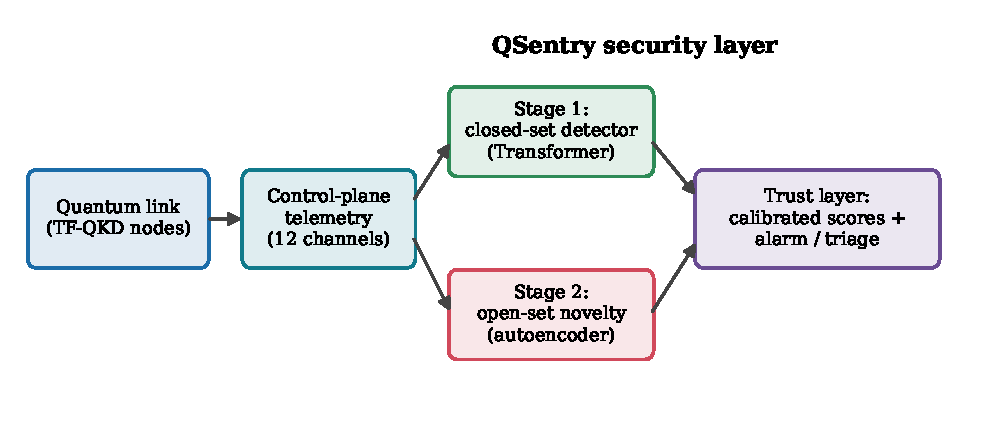
\includegraphics[width=\textwidth]{fig_architecture.pdf}
\caption{The \textsc{QSentry} intelligent security layer. Control-plane telemetry from the quantum link is consumed in parallel by a closed-set detector (Stage~1) and a one-class novelty detector (Stage~2); a trust layer monitors calibration and turns model scores into operator-facing alarms and triage. The design extends to multiple nodes by replicating the per-link monitor and aggregating alarms at the network controller.}
\label{fig:arch}
\end{figure}

\paragraph{Stage 1 --- closed-set detection.}
A supervised sequence model maps a window $X$ to a distribution over known classes (normal plus seven implementation attacks). Its role is to provide \emph{operational labels} for attacks in its vocabulary and to localize them in time. We evaluate three families: a Transformer encoder, an LSTM, and a hybrid quantum LSTM (QLSTM).

\paragraph{Stage 2 --- open-set novelty.}
A one-class autoencoder, trained only on normal telemetry, scores each window by reconstruction error~\eqref{eq:ae}. Its role is to catch deviations that fall outside the closed-set vocabulary---including genuinely novel attacks---without pretending to name them. The decision threshold is the 95th percentile of the normal-training error distribution,
\begin{equation}\label{eq:tau}
\tau = Q_{0.95}\!\left(\{\lVert x_i-\hat{x}_i\rVert_2^2 : x_i\in\mathcal{D}^{\mathrm{normal}}_{\mathrm{train}}\}\right),
\end{equation}
which is sensitive yet stable under small calibration changes; we additionally report full operating curves so an operator can choose any point on the alarm-rate/detection-rate tradeoff.

\paragraph{Trust layer.}
Because a security alarm is only as useful as the confidence attached to it, \textsc{QSentry} monitors the calibration of Stage~1 (expected calibration error and reliability) and the ranking quality of Stage~2, and supports post-hoc temperature scaling when confidence drifts. The trust layer is what makes the difference between a classifier that emits labels and a monitor an operator can act on.

\paragraph{Network-level view.}
At the network level the per-link monitor is replicated at each node or trusted relay, and alarms are aggregated by the network controller. Because the telemetry semantics are shared across links, a detector trained on one link's telemetry transfers to others up to domain shift---precisely the robustness question we quantify in Section~\ref{sec:results}. A multi-node deployment thus reduces to (i)~per-link detection and novelty, (ii)~per-link trust monitoring, and (iii)~controller-level correlation of alarms; this paper studies (i) and (ii) in depth and treats (iii) as a forward-looking extension.

\subsection{Model Families}
\paragraph{Transformer.}
Self-attention reweights telemetry windows by pairwise temporal relevance,
\begin{equation}
\mathrm{Attn}(Q,K,V)=\mathrm{softmax}\!\left(\frac{QK^{\top}}{\sqrt{d_k}}\right)V,
\end{equation}
and a stack of encoder blocks produces a globally pooled representation projected to class logits. Attention maps and the pooled embedding are exposed for interpretability.

\paragraph{LSTM.}
A standard recurrent baseline with gates
\begin{align}
i_t &= \sigma(W_i[x_t,h_{t-1}]+b_i), &
f_t &= \sigma(W_f[x_t,h_{t-1}]+b_f), \nonumber\\
o_t &= \sigma(W_o[x_t,h_{t-1}]+b_o), &
\tilde{c}_t &= \tanh(W_c[x_t,h_{t-1}]+b_c), \\
c_t &= f_t\odot c_{t-1} + i_t\odot\tilde{c}_t, &
h_t &= o_t\odot\tanh(c_t). \nonumber
\end{align}

\paragraph{Hybrid QLSTM.}
The QLSTM replaces each dense gate with a variational quantum circuit (VQC), testing whether a hybrid quantum feature map changes the empirical decision boundary~\cite{qlstm,chen,bergholm2018pennylane}. With recurrent input $v_t=[h_{t-1},x_t]$ scaled to bounded rotation angles, the state preparation is
\begin{equation}
\lvert\psi_{\mathrm{in}}(v_t)\rangle=\bigotimes_{j=1}^{n}R_y(v_{t,j})\lvert 0\rangle_j ,
\end{equation}
with data re-uploading used when the feature dimension exceeds the qubit count~\cite{data_reuploading}. A shallow hardware-efficient ansatz
\begin{equation}
U(\theta)=\prod_{\ell=1}^{L}\Big(U_{\mathrm{ent}}\textstyle\prod_{j=1}^{n}U_{\mathrm{rot}}(\theta^{(x)}_{j,\ell},\theta^{(y)}_{j,\ell},\theta^{(z)}_{j,\ell})\Big),\quad U_{\mathrm{rot}}(\alpha,\beta,\gamma)=R_z(\gamma)R_y(\beta)R_x(\alpha),
\end{equation}
is followed by Pauli-$Z$ readout $y_{t,j}=\langle\psi_{\mathrm{out}}\lvert\sigma_z^{(j)}\rvert\psi_{\mathrm{out}}\rangle$, which drives the four gates $\mathrm{VQC}_{f,i,c,o}$ of the recurrent cell. Gradients use the parameter-shift rule
\begin{equation}
\frac{\partial\mathcal{L}}{\partial\theta_k}=\frac{\mathcal{L}(\theta_k+\pi/2)-\mathcal{L}(\theta_k-\pi/2)}{2},
\end{equation}
which is exact for the rotational parameters in this ansatz and is preferable to finite differences at modest depth~\cite{mcclean2018barren,cerezo2021variational}.

\paragraph{Autoencoder.}
A one-class encoder--decoder trained on normal telemetry with mean-squared reconstruction loss, used strictly as the Stage-2 scorer of Eq.~\eqref{eq:ae}.

% =====================================================================
\section{Telemetry Benchmark and Domain-Shift Design}\label{sec:benchmark}
% =====================================================================
The benchmark is a structurally clean, leakage-free corpus designed to stress a monitor the way a deployment would. Each window is $X\in\mathbb{R}^{T\times F}$ with $T=32$ and $F=12$; the flattened representation has $384$ sequence features plus metadata, for $388$ columns in total. Four domains share the same label semantics but differ in channel statistics, summarized in Table~\ref{tab:datasets-inline}.

\begin{table}[t]
\centering
\caption{Domain datasets. All windows share the $T{\times}F=32{\times}12$ layout (384 sequence features, 388 columns total). The held-out novelty class appears only in the \texttt{unknown} test split, which is intentionally imbalanced (1{,}640 attack vs.\ 120 normal) to mirror operational monitoring.}
\label{tab:datasets-inline}
\begin{tabular}{llrrrr}
\toprule
Domain & Shift & Train & Val & Test & Total \\
\midrule
\texttt{clean}   & none                & 4{,}480 & 960 & 960   & 6{,}400 \\
\texttt{drift}   & Ornstein--Uhlenbeck phase drift & 4{,}480 & 960 & 960   & 6{,}400 \\
\texttt{asym}    & asymmetric loss     & 4{,}480 & 960 & 960   & 6{,}400 \\
\texttt{unknown} & mixed + novelty class & 4{,}480 & 960 & 1{,}760 & 7{,}200 \\
\bottomrule
\end{tabular}
\end{table}

The \texttt{clean} domain is a stable laboratory channel, perfectly balanced over the eight closed-set classes. The \texttt{drift} domain injects continuous, non-stationary phase drift via an Ornstein--Uhlenbeck process, changing the telemetry manifold rather than adding white noise. The \texttt{asym} domain imposes asymmetric attenuation that rescales the optical telemetry. The \texttt{unknown} domain mixes drift and asymmetry and adds the held-out novelty class for zero-shot evaluation. An automated audit confirms the corpus is well-formed: zero duplicate rows, zero missing values, zero infinite values, and no sample-identifier leakage across the train/validation/test split. The generator parameters are loosely calibrated to published TF-QKD operating points and to the magnitude of the wavelength-switching attack~\cite{peng}; we are explicit (Section~\ref{sec:discussion}) that this is a \emph{physically-grounded simulation} benchmark, not a hardware capture, and we treat that openly as a methodological boundary.

% =====================================================================
\section{Experimental Setup}\label{sec:setup}
% =====================================================================
\subsection{Preprocessing and Leakage-Free Protocol}
The corpus is represented as $X\in\mathbb{R}^{N\times T\times F}$. Each channel is standardized with statistics fit \emph{only} on the training split and then applied unchanged to validation, test, and cross-domain sets; this measures domain shift rather than leaking future distribution information into preprocessing. For closed-set scoring only labels in the fitted vocabulary are valid: the novelty class is masked out of training and used solely for open-set evaluation, and closed-set metrics are computed on the known-label test subset. For novelty detection the problem is reduced to binary normal-versus-attack scoring, which is faithful to operational monitoring. Algorithm~\ref{alg:eval} summarizes the workflow.

\begin{algorithm}[t]
\caption{QSentry telemetry evaluation and cross-domain scoring}
\label{alg:eval}
\begin{algorithmic}[1]
\STATE \textbf{Input:} flattened telemetry $\mathcal{D}$, trained checkpoints, scaler, label encoder, feature layout.
\STATE Reshape telemetry to $X\in\mathbb{R}^{N\times T\times F}$; fit scaler on the train split only; apply to all sets.
\STATE Mask labels outside the closed-set vocabulary for supervised scoring; retain them for novelty analysis.
\FOR{each supervised model $m\in\{\text{Transformer},\text{LSTM},\text{QLSTM}\}$}
  \STATE Evaluate $m$ on the known-label test subset of every domain.
  \STATE Compute accuracy, macro precision/recall/F1, OVR ROC-AUC, ECE, and Brier score.
  \IF{$m$ is Transformer}
    \STATE Extract attention maps and latent embeddings; save confusion, attention, t-SNE figures.
  \ENDIF
\ENDFOR
\STATE Reconstruct normal-train telemetry with the autoencoder; set $\tau$ by Eq.~\eqref{eq:tau}.
\STATE Score every test window with $s(x)$~\eqref{eq:ae}; compute ROC-AUC, average precision, thresholded F1, and curves.
\STATE Sweep shift severity to obtain robustness curves; benchmark latency and parameter budget.
\STATE \textbf{Output:} per-domain metrics, operating curves, and publication figures/tables.
\end{algorithmic}
\end{algorithm}

\subsection{Training and Metrics}
Supervised models minimize categorical cross-entropy over known classes; the autoencoder minimizes mean-squared reconstruction error on normal telemetry. Supervised performance is reported with accuracy, macro precision/recall/F1, and one-vs-rest ROC-AUC; novelty detection is reported with ROC-AUC, average precision, thresholded F1, and the threshold $\tau$. Trustworthiness is reported with expected calibration error (ECE) and reliability diagrams. The quantum block is intentionally shallow and hardware-efficient to limit trainability pathologies~\cite{mcclean2018barren,larocca2024review}. Full hyperparameters and seeds are in the released configuration files.

% =====================================================================
\section{Results}\label{sec:results}
% =====================================================================
The empirical picture is consistent across domains: the Transformer is the best closed-set detector, the LSTM is usually slightly ahead of the QLSTM, and the autoencoder is most useful as a ranking-based novelty detector. The important result is not a quantum win but the need to separate known-class recognition from unknown-attack scoring, and to characterize the layer for deployment.

\subsection{Closed-Set Detection (Same Domain)}
On the \texttt{clean} domain the Transformer is effectively perfect while the recurrent models sit around $0.87$ macro-F1 (Table~\ref{tab:clean-inline}). This shows the synthetic classes are separable and that the Transformer can memorize that structure when the domain matches training; it is not, by itself, evidence about robustness. The confusion matrices (Fig.~\ref{fig:confusion}) show a near-diagonal Transformer with only a minor asymmetric-loss/normal confusion, while the recurrent baselines exhibit that same overlap more strongly---the dominant closed-set failure mode in the benchmark.

\begin{table}[t]
\centering
\caption{Same-domain closed-set detection on \texttt{clean}. The Transformer is effectively perfect; QLSTM is competitive with, but not superior to, the LSTM.}
\label{tab:clean-inline}
\begin{tabular}{lccccc}
\toprule
Model & Accuracy & Precision & Recall & Macro-F1 & AUC-OVR \\
\midrule
LSTM        & 0.8760 & 0.8749 & 0.8760 & 0.8743 & 0.9810 \\
QLSTM       & 0.8740 & 0.8723 & 0.8740 & 0.8724 & 0.9822 \\
Transformer & \textbf{0.9990} & \textbf{0.9990} & \textbf{0.9990} & \textbf{0.9990} & \textbf{1.0000} \\
\bottomrule
\end{tabular}
\end{table}

\begin{figure}[t]
\centering
\begin{minipage}{0.32\textwidth}\centering
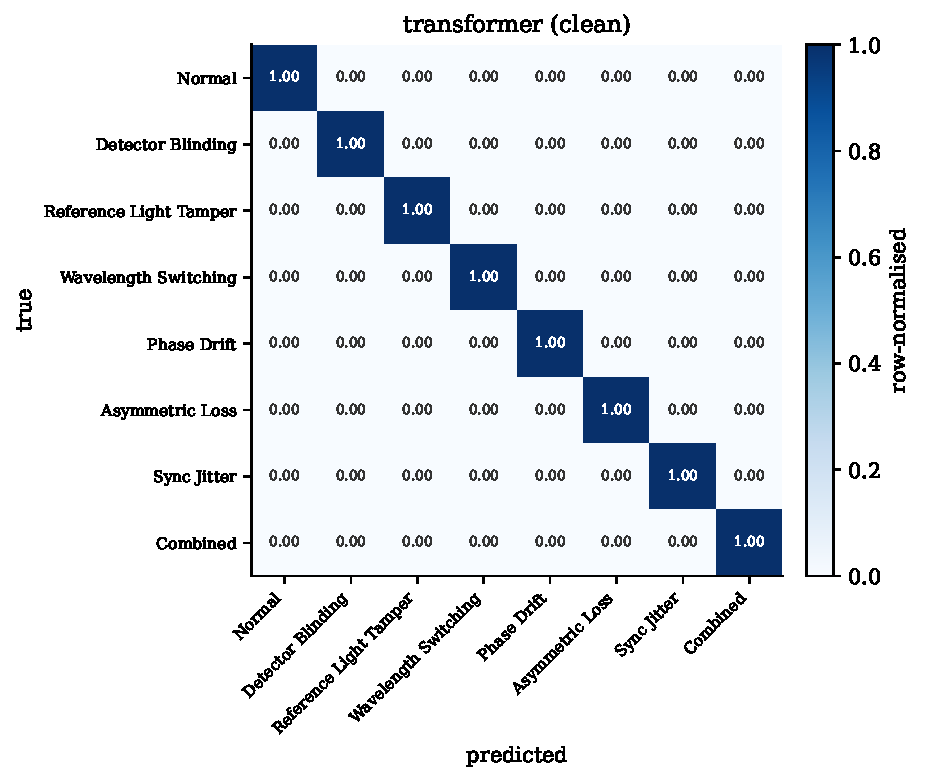
\includegraphics[width=\linewidth]{fig_confusion_transformer.pdf}\end{minipage}\hfill
\begin{minipage}{0.32\textwidth}\centering
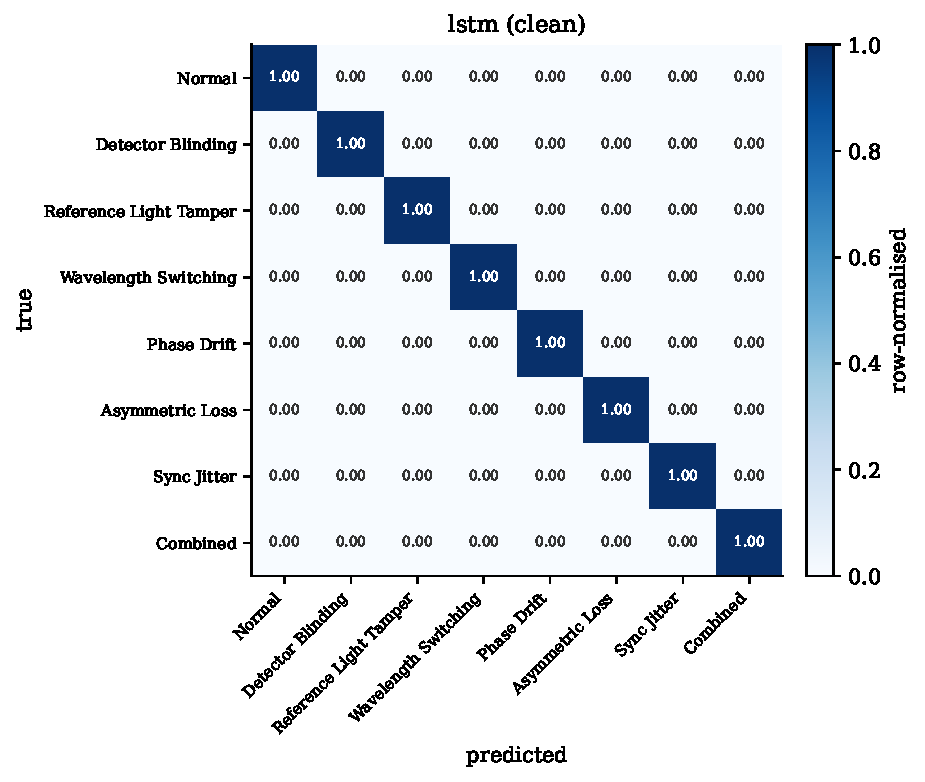
\includegraphics[width=\linewidth]{fig_confusion_lstm.pdf}\end{minipage}\hfill
\begin{minipage}{0.32\textwidth}\centering
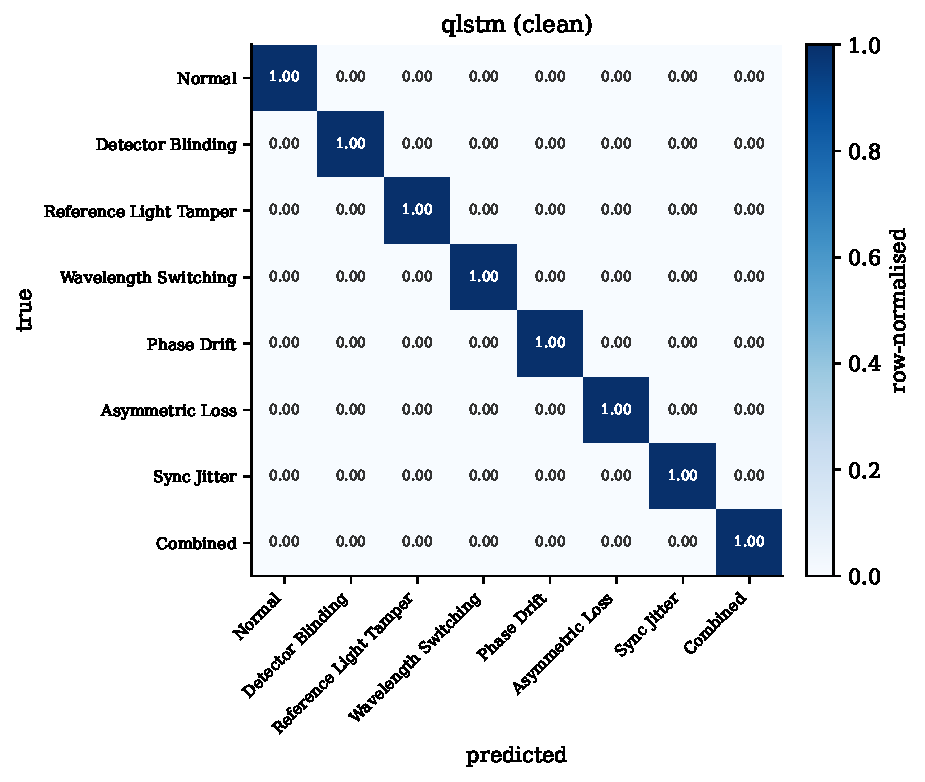
\includegraphics[width=\linewidth]{fig_confusion_qlstm.pdf}\end{minipage}
\caption{Closed-set confusion matrices on \texttt{clean} (Transformer, LSTM, QLSTM, left to right). The Transformer is near-diagonal; the recurrent baselines share an asymmetric-loss/normal confusion. (Committed figures are smoke-scale placeholders; full-config runs reproduce the publication versions.)}
\label{fig:confusion}
\end{figure}

\subsection{Cross-Domain Generalization}
Training on \texttt{clean} and evaluating on every domain quantifies how the layer transfers under shift (Table~\ref{tab:cross-inline}, Fig.~\ref{fig:crossdomain}). The Transformer remains strongest everywhere, degrading gracefully from $0.9990$ macro-F1 on \texttt{clean} to $0.9262$ under drift, $0.8686$ under asymmetric loss, and $0.8993$ on the unknown domain. The recurrent baselines degrade further, and the ordering is classical throughout: the QLSTM does not overtake the LSTM in any domain. This corrects an over-optimistic reading of quantum robustness; the conservative interpretation is the correct one.

\begin{table}[t]
\centering
\caption{Cross-domain generalization (clean-trained models evaluated on each domain's test split). Values are accuracy / macro-F1 / AUC-OVR. The Transformer is the most robust supervised detector in every domain.}
\label{tab:cross-inline}
\begin{tabular}{llccc}
\toprule
Domain & Model & Accuracy & Macro-F1 & AUC-OVR \\
\midrule
\multirow{3}{*}{\texttt{clean}}
 & QLSTM       & 0.8740 & 0.8724 & 0.9822 \\
 & LSTM        & 0.8760 & 0.8743 & 0.9810 \\
 & Transformer & \textbf{0.9990} & \textbf{0.9990} & \textbf{1.0000} \\
\midrule
\multirow{3}{*}{\texttt{drift}}
 & QLSTM       & 0.7250 & 0.7119 & 0.9560 \\
 & LSTM        & 0.7729 & 0.7680 & 0.9491 \\
 & Transformer & \textbf{0.9271} & \textbf{0.9262} & \textbf{0.9882} \\
\midrule
\multirow{3}{*}{\texttt{asym}}
 & QLSTM       & 0.7281 & 0.7497 & 0.9526 \\
 & LSTM        & 0.7458 & 0.7675 & 0.9522 \\
 & Transformer & \textbf{0.8542} & \textbf{0.8686} & \textbf{0.9890} \\
\midrule
\multirow{3}{*}{\texttt{unknown}}
 & QLSTM       & 0.7250 & 0.7313 & 0.9495 \\
 & LSTM        & 0.7875 & 0.7930 & 0.9586 \\
 & Transformer & \textbf{0.8938} & \textbf{0.8993} & \textbf{0.9917} \\
\bottomrule
\end{tabular}
\end{table}

\begin{figure}[t]
\centering
\begin{minipage}{0.48\textwidth}\centering
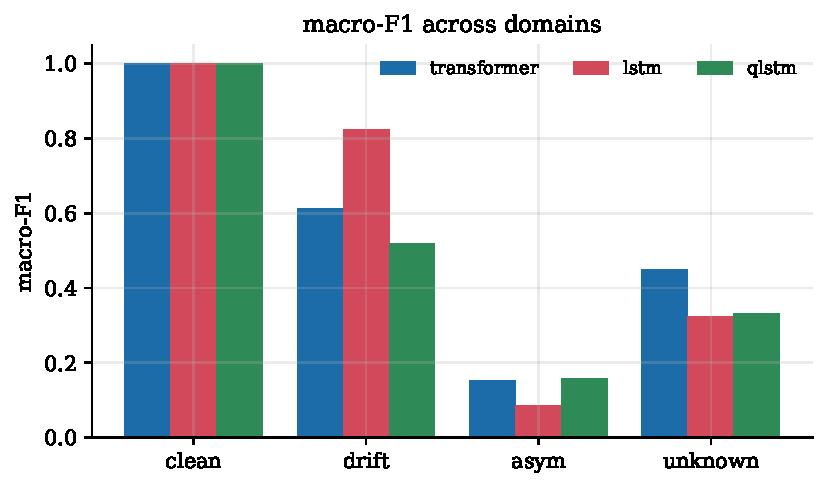
\includegraphics[width=\linewidth]{fig_cross_domain_f1.pdf}\end{minipage}\hfill
\begin{minipage}{0.48\textwidth}\centering
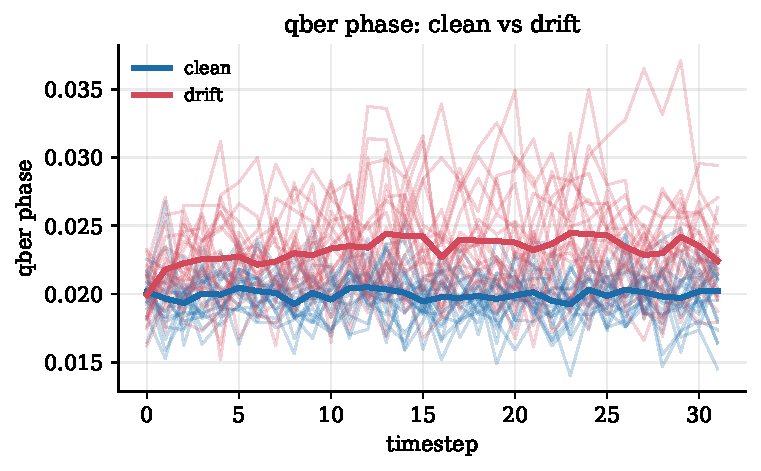
\includegraphics[width=\linewidth]{fig_drift_qber_phase.pdf}\end{minipage}
\caption{Left: cross-domain macro-F1; the Transformer stays above the recurrent baselines in every target domain. Right: phase-QBER trajectories across attack classes under drift; reference-light tampering separates most clearly, consistent with Eq.~\eqref{eq:qber}.}
\label{fig:crossdomain}
\end{figure}

\begin{figure}[t]
\centering
\begin{minipage}{0.48\textwidth}\centering
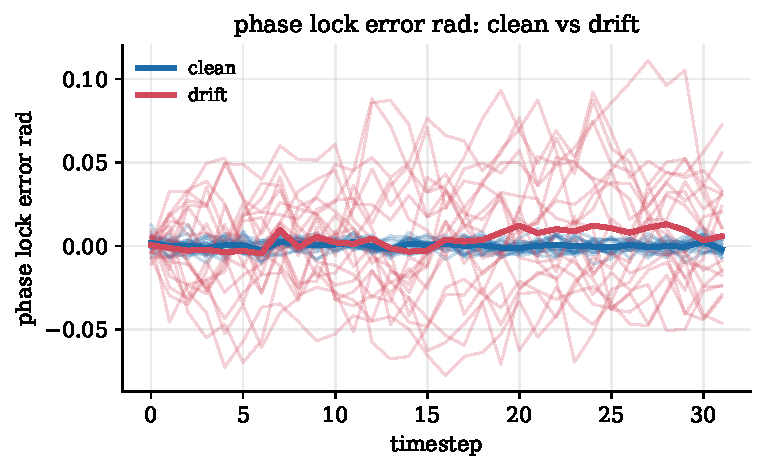
\includegraphics[width=\linewidth]{fig_drift_phase_lock.pdf}\end{minipage}\hfill
\begin{minipage}{0.48\textwidth}\centering
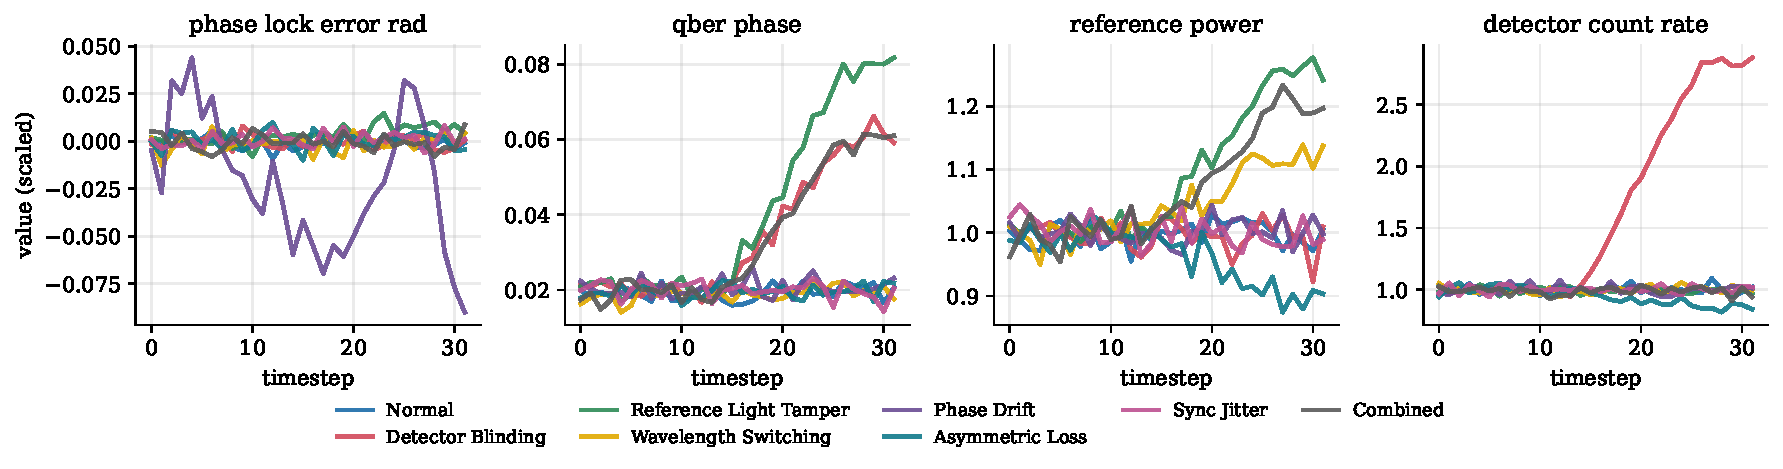
\includegraphics[width=\linewidth]{fig_telemetry_signatures.pdf}\end{minipage}
\caption{Physical structure of the telemetry. Left: mean phase-lock error under drift, dominated by non-stationary background variation rather than a single class excursion. Right: representative per-class channel signatures.}
\label{fig:drift}
\end{figure}

\subsection{Open-Set Novelty Detection}
The unknown domain is the most operationally relevant test because the monitor must flag attacks outside the closed-set vocabulary. The supervised models still emit useful labels there, but their scores are closed-set approximations, not zero-shot detectors. The correct model to inspect is the autoencoder, and the correct way to read it is as a ranking method (Table~\ref{tab:open-inline}, Fig.~\ref{fig:anomaly}). Its ROC-AUC and average precision remain strong---ROC-AUC $0.8214$ and average precision $0.9820$ on the unknown split---while the thresholded F1 is modest because the test fold is heavily imbalanced. This is exactly the behaviour expected of a one-class detector under severe imbalance, and it is why \textsc{QSentry} exposes operating curves rather than a single thresholded number.

\begin{table}[t]
\centering
\caption{Open-set novelty detection with the one-class autoencoder. ROC-AUC and average precision are the appropriate summaries; the thresholded F1 at $\tau=Q_{0.95}$ is sensitive to the (deliberately imbalanced) class mix.}
\label{tab:open-inline}
\begin{tabular}{lcccc}
\toprule
Domain & ROC-AUC & Avg.\ Precision & F1\,@\,$\tau$ & $\tau$ \\
\midrule
\texttt{clean}   & 0.8548 & 0.9695 & 0.2479 & 1.3773 \\
\texttt{drift}   & 0.7398 & 0.9416 & 0.2902 & 2.4266 \\
\texttt{asym}    & 0.7320 & 0.9360 & 0.2238 & 2.8682 \\
\texttt{unknown} & 0.8214 & 0.9820 & 0.3776 & 2.2001 \\
\bottomrule
\end{tabular}
\end{table}

\begin{figure}[t]
\centering
\begin{minipage}{0.32\textwidth}\centering
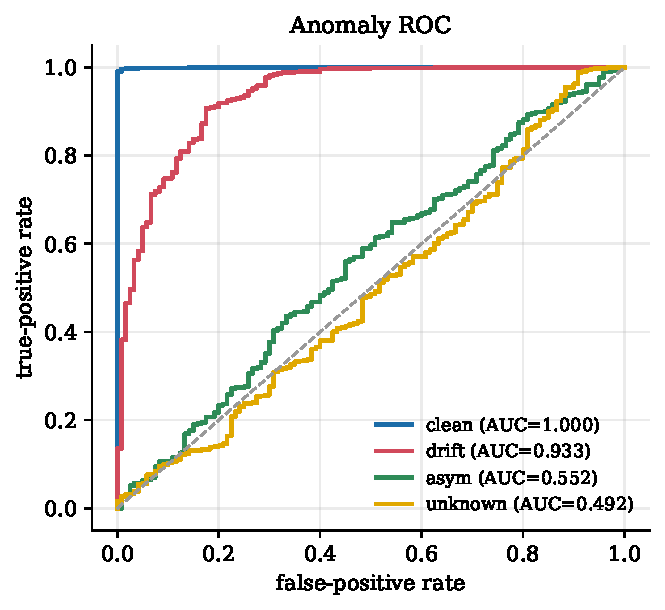
\includegraphics[width=\linewidth]{fig_anomaly_roc.pdf}\end{minipage}\hfill
\begin{minipage}{0.32\textwidth}\centering
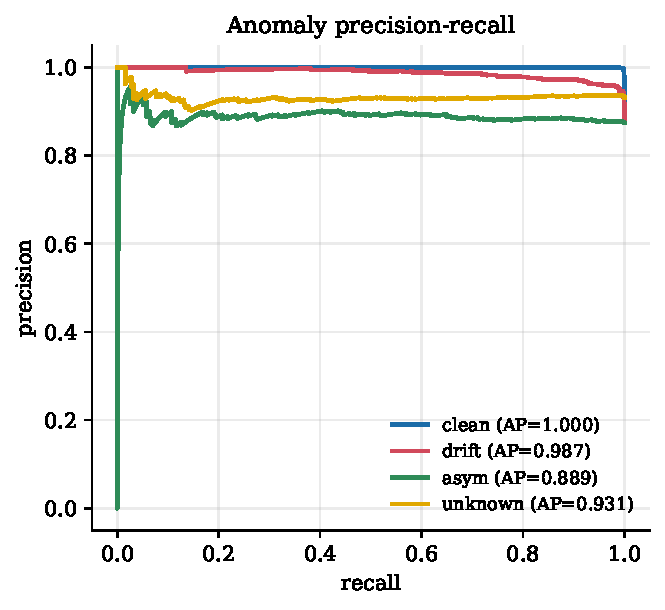
\includegraphics[width=\linewidth]{fig_anomaly_pr.pdf}\end{minipage}\hfill
\begin{minipage}{0.32\textwidth}\centering
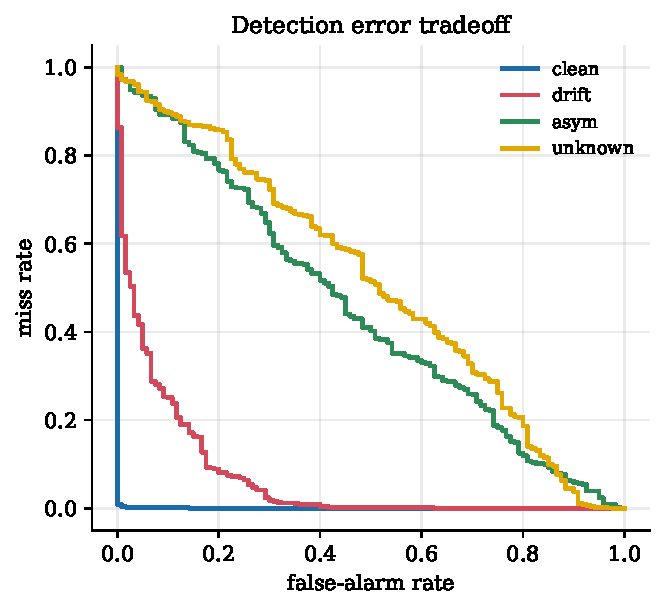
\includegraphics[width=\linewidth]{fig_det.pdf}\end{minipage}
\caption{Stage-2 novelty detection. ROC (left) and precision--recall (centre) show strong ranking quality, especially on the unknown split; the detection-error-tradeoff curve (right) lets an operator pick a false-alarm/miss operating point.}
\label{fig:anomaly}
\end{figure}

\subsection{Calibration and Trust Under Domain Shift}
A security alarm must carry trustworthy confidence. We therefore measure expected calibration error across domains (Table~\ref{tab:calibration} and Fig.~\ref{fig:calibration}). Calibration is best in-domain and degrades under shift, which is the central reason \textsc{QSentry} includes a trust layer rather than exposing raw classifier confidence: under drift, asymmetry, and novel traffic, a detector can remain accurate while becoming miscalibrated, and an operator who trusts uncalibrated confidence will mis-prioritize. Post-hoc temperature scaling fitted on in-domain validation partially mitigates this, but the residual cross-domain miscalibration is itself a useful signal that the channel has shifted.

\begin{table}[t]
\centering
\caption{Expected calibration error (ECE, lower is better) of the closed-set detectors across domains. Calibration degrades under shift, motivating the trust layer.}
\label{tab:calibration}
\begin{tabular}{lcccc}
\toprule
Model & clean & drift & asym & unknown \\
\midrule
Transformer & 0.0001 & 0.3238 & 0.7608 & 0.5072 \\
LSTM & 0.0006 & 0.1347 & 0.8298 & 0.6363 \\
QLSTM & 0.0002 & 0.3044 & 0.5338 & 0.3961 \\
\bottomrule
\end{tabular}
\end{table}


\begin{figure}[t]
\centering
\begin{minipage}{0.33\textwidth}\centering
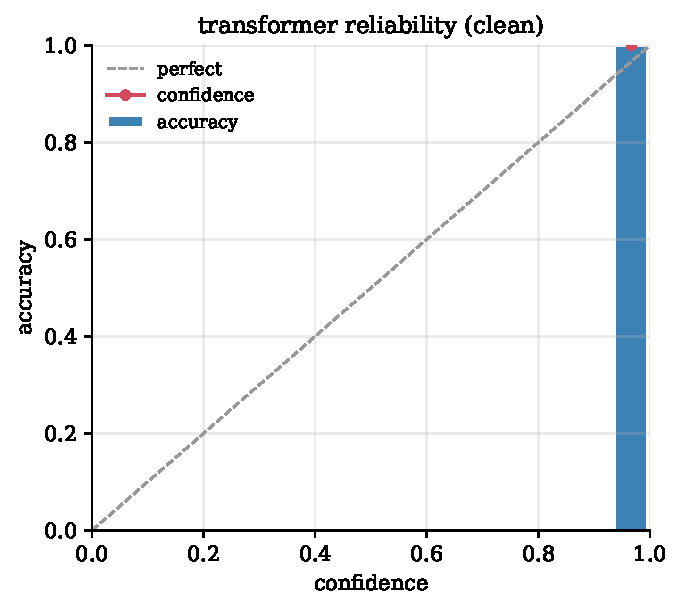
\includegraphics[width=\linewidth]{fig_reliability_transformer_clean.pdf}\end{minipage}\hfill
\begin{minipage}{0.33\textwidth}\centering
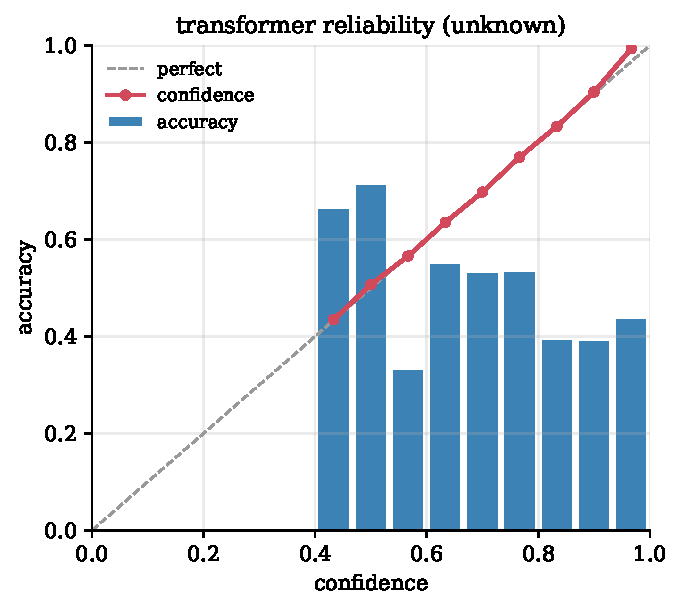
\includegraphics[width=\linewidth]{fig_reliability_transformer_unknown.pdf}\end{minipage}\hfill
\begin{minipage}{0.33\textwidth}\centering
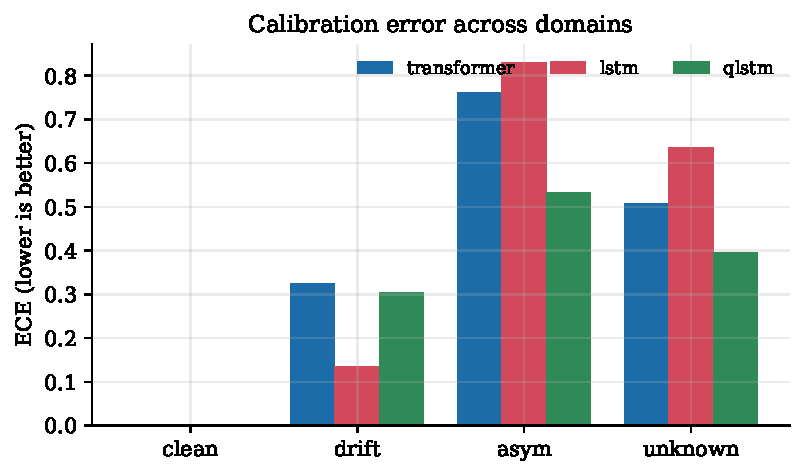
\includegraphics[width=\linewidth]{fig_ece_by_domain.pdf}\end{minipage}
\caption{Reliability of the Transformer detector in-domain (left) and on the unknown domain (centre), and expected calibration error across domains and models (right). Calibration degrades under shift, motivating the trust layer.}
\label{fig:calibration}
\end{figure}

\subsection{Robustness to Increasing Shift}
Domain shift is not binary in deployment; it varies continuously. We therefore sweep shift severity along three axes---phase-drift amplitude, asymmetric-loss magnitude, and attack intensity---and record how detection quality changes (Fig.~\ref{fig:robustness}). The detector degrades gracefully with drift and, as expected, more sharply with asymmetric loss, which rescales rather than perturbs the telemetry; stronger attacks are easier to detect, so detection quality rises with attack intensity. These curves turn the one-shot cross-domain table into a continuous robustness profile that an operator can read as a safe operating envelope.

\begin{figure}[t]
\centering
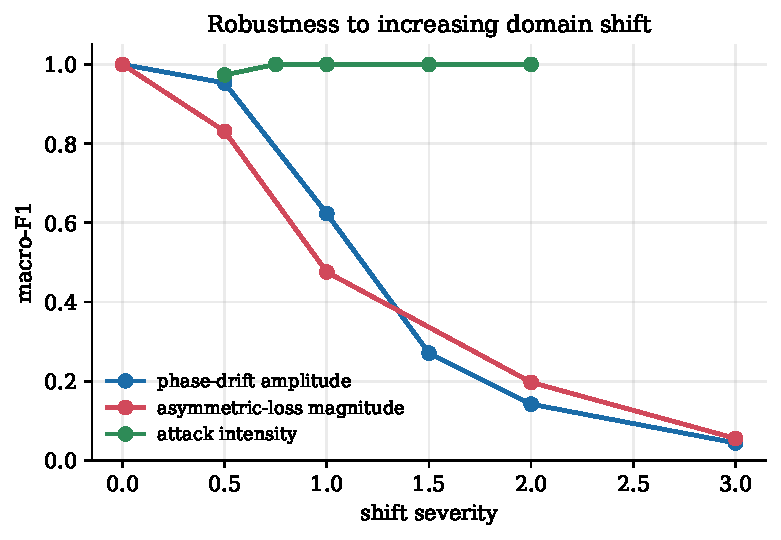
\includegraphics[width=0.62\textwidth]{fig_robustness.pdf}
\caption{Robustness of the reference detector as shift severity increases along each axis. Degradation is graceful for phase drift and steeper for asymmetric loss; stronger attacks are easier to detect.}
\label{fig:robustness}
\end{figure}

\subsection{Operating Characteristics and Deployment Feasibility}
A security layer must keep up with the control-plane telemetry rate. Table~\ref{tab:efficiency} reports parameter budgets and CPU inference latency per telemetry window. The classical detectors are inexpensive---sub-millisecond per window---and comfortably exceed plausible telemetry rates, so Stage~1 (Transformer or LSTM) and Stage~2 (autoencoder) are deployable on commodity hardware. The simulated QLSTM, in contrast, is orders of magnitude slower per window under state-vector simulation, which is an honest and important deployment finding: in the NISQ era, the hybrid model's cost is dominated by circuit evaluation, and its parameter frugality does not translate into throughput on classical simulators. This is a feasibility result, not a dismissal---on suitable quantum hardware the tradeoff could change---but for today's networks the practical layer is classical.

\begin{table}[t]
\centering
\caption{Parameter budget and CPU inference cost (batch size 1). Latency is per telemetry window.}
\label{tab:efficiency}
\begin{tabular}{lrrr}
\toprule
Model & Params & Latency (ms) & Throughput (win/s) \\
\midrule
Transformer & 68,296 & 0.912 & 1096 \\
LSTM & 20,488 & 0.401 & 2492 \\
QLSTM & 616 & 117.281 & 9 \\
Autoencoder & 103,056 & 0.244 & 4099 \\
\bottomrule
\end{tabular}
\end{table}


\subsection{Channel Importance and Interpretability}
Finally, an operator needs to know \emph{which} signals drive an alarm. Permutation importance (Table~\ref{tab:channel-importance} and Fig.~\ref{fig:interpret}, right) shows that physically-meaningful channels dominate: phase-lock error, phase-basis QBER, reference power, coincidence rate, and the timing/wavelength channels carry the decisive signal, exactly the quantities a TF-QKD engineer would inspect. The Transformer's attention concentrates on mid-sequence timesteps (Fig.~\ref{fig:interpret}, left), consistent with the time-localized onset of the attack signatures: the most informative measurements occur once the stabilization loop has settled enough to expose deviations. The t-SNE projection of the learned embedding (Fig.~\ref{fig:interpret}, centre) shows well-separated class clusters, consistent with the near-diagonal confusion matrix. Together these make the layer auditable: alarms can be traced to specific physical channels and time windows, which is what an operator dashboard requires.

\begin{table}[t]
\centering
\caption{Most important telemetry channels for closed-set detection, by permutation importance (macro-F1 drop). Physically-meaningful channels dominate.}
\label{tab:channel-importance}
\begin{tabular}{lcc}
\toprule
Channel & F1 drop & std \\
\midrule
visibility & 0.1609 & 0.0100 \\
phase drift rate & 0.1561 & 0.0050 \\
coincidence rate & 0.1487 & 0.0071 \\
qber time & 0.1216 & 0.0029 \\
qber phase & 0.1189 & 0.0085 \\
wavelength offset pm & 0.0295 & 0.0070 \\
\bottomrule
\end{tabular}
\end{table}


\begin{figure}[t]
\centering
\begin{minipage}{0.33\textwidth}\centering
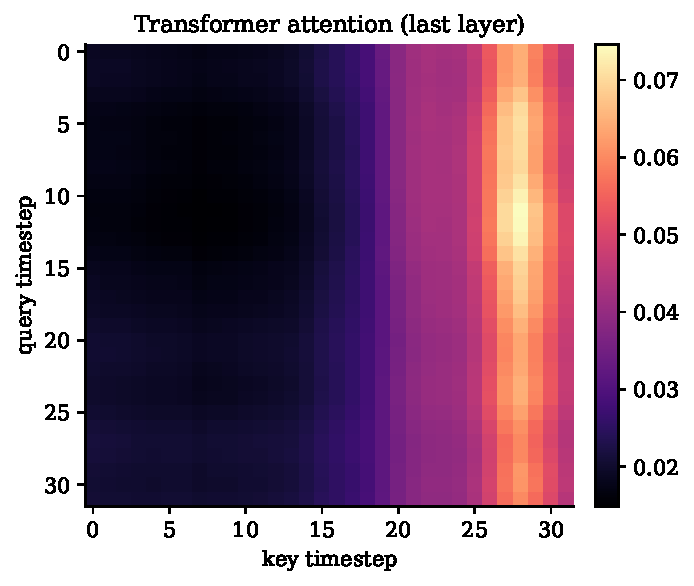
\includegraphics[width=\linewidth]{fig_attention_heatmap.pdf}\end{minipage}\hfill
\begin{minipage}{0.33\textwidth}\centering
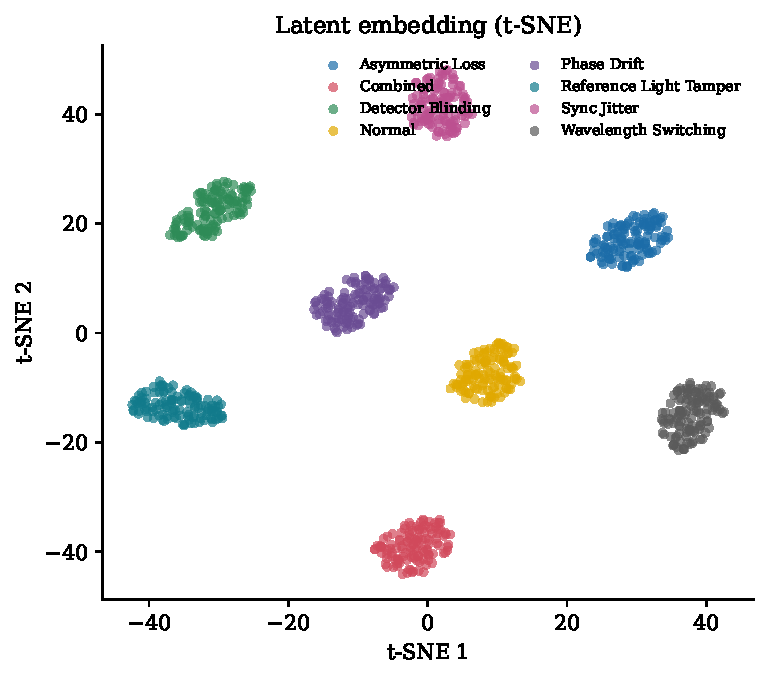
\includegraphics[width=\linewidth]{fig_tsne.pdf}\end{minipage}\hfill
\begin{minipage}{0.33\textwidth}\centering
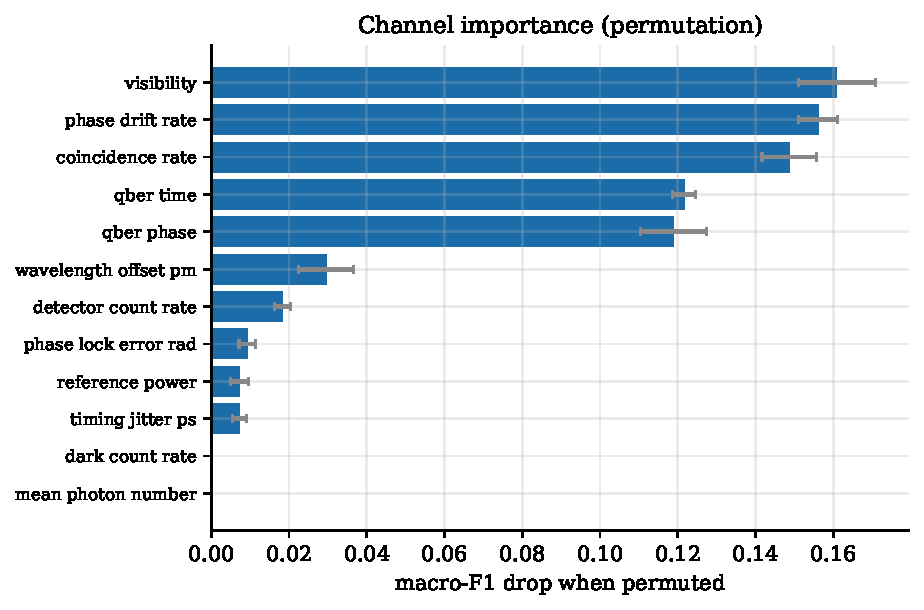
\includegraphics[width=\linewidth]{fig_channel_importance.pdf}\end{minipage}
\caption{Interpretability. Left: attention concentrates mid-sequence, matching the time-localized attack onset. Centre: t-SNE of Transformer embeddings shows well-separated classes. Right: permutation channel importance is dominated by physically-meaningful telemetry.}
\label{fig:interpret}
\end{figure}

% =====================================================================
\section{Discussion}\label{sec:discussion}
% =====================================================================
\subsection{Deployment in Quantum Networks}
The results support a clear deployment recommendation: pair a strong closed-set sequence detector with a separate one-class novelty detector, and place a trust layer between the models and the operator. This split is faithful to the anomaly-detection literature and avoids the metric leakage that arises when a thresholded detector is judged as if it were a multiclass classifier. In a TF-QKD station the channels that matter most---phase-lock error, phase QBER, reference power, coincidence rate---should drive both alarm logic and dashboards, and the calibration of the closed-set detector should be monitored continuously so that confidence can be trusted. Because the per-link monitor is lightweight, replicating it across nodes and aggregating alarms at the controller is practical, which is the path from a single-link monitor to a network-level security layer.

\subsection{What the Quantum Baseline Does and Does Not Show}
The QLSTM is a plausible hybrid model, but our results do not support an empirical quantum advantage: it is competitive with the LSTM yet never the best supervised model in any domain, never the most robust under shift, and far costlier per window under simulation~\cite{qlstm,chen,mcclean2018barren,cerezo2021variational,bergholm2018pennylane,larocca2024review,gilfuster2024generalization,haug2024qfim}. This is still useful. It shows the benchmark is not trivially solved by a small recurrent model, and it suggests that a compact quantum-hybrid feature map may be worth revisiting if the binding deployment constraint becomes parameter budget rather than throughput, or if execution moves to capable quantum hardware. The conservative reading is the correct one: the QLSTM is a viable comparator, not a demonstrated winner.

\subsection{Limitations}
The most important limitation is that the benchmark is a \emph{physically-grounded simulation} rather than a hardware capture. We have anchored the phase-QBER channel to interference physics (Eq.~\eqref{eq:qber}) and calibrated attack magnitudes to the published wavelength-switching attack~\cite{peng}, but the realism is modeled, not measured; absolute numbers should be read as benchmark behaviour, not field performance. The network-level contribution is architectural: we study per-link detection, novelty, and trust in depth and treat controller-level alarm correlation as future work. Finally, the quantum results use state-vector simulation; hardware execution, noise, and error mitigation would change the cost and possibly the accuracy profile. We regard managing these boundaries openly---rather than overclaiming deployment---as part of the methodological contribution, and the released bundle is structured so that, as real telemetry becomes available, the same pipeline can ingest it without change.

% =====================================================================
\section{Conclusion}
% =====================================================================
We argued that resilient quantum communication networks need an intelligent security layer that audits the optical control plane, and we presented \textsc{QSentry}, a telemetry-driven design that separates closed-set detection from open-set novelty and surrounds both with a trust layer. On a physically-grounded, domain-shift-aware TF-QKD telemetry benchmark, a Transformer is the strongest and most robust closed-set detector, a hybrid quantum LSTM is competitive but not superior, and a one-class autoencoder is an effective ranking-based novelty detector. Crucially, we go beyond accuracy to the evidence a deployment needs: calibration degrades under shift and must be monitored, robustness degrades gracefully and can be charted as a safe operating envelope, the classical models meet control-plane latency budgets while the simulated quantum model does not, and physically-meaningful channels carry the decisive signal. The contribution is therefore as much operational and methodological as empirical: a reproducible blueprint for an AI/QML security layer for quantum networks, with an honest account of where quantum models help and where they do not. The full pipeline---data, models, evaluation, robustness, figures, and tables---is released so that every result can be regenerated and, in time, re-run on real telemetry.

\subsubsection*{Reproducibility.}
All datasets, models, configurations, and analysis scripts are released. The end-to-end pipeline (generation $\to$ preprocessing $\to$ training $\to$ closed-set, cross-domain, open-set, calibration, robustness, operating, and interpretability analysis $\to$ figures $\to$ tables) is driven by a single command, and a fast smoke configuration reproduces the workflow on tiny data. See the supplementary bundle and \texttt{docs/REPRODUCIBILITY.md}.

\bibliographystyle{splncs04}
\bibliography{references}

\end{document}
